\documentclass[12pt,addpoints]{repaso}
\grado{3}
\nivel{Primaria}
\cicloescolar{2024-2025}
\materia{Matemáticas}
\unidad{3}
\title{Practica la Unidad}
\aprendizajes{\scriptsize%
\item Expresa oralmente la sucesión numérica hasta cuatro cifras, en español y hasta donde sea posible, en su lengua materna, de manera ascendente y descendente a partir de un número natural dado.\\[-1.8em]
\item Representa, con apoyo de material concreto y modelos gráficos, fracciones: medios, cuartos, octavos, dieciseisavos, para expresar el resultado de mediciones y repartos en situaciones vinculadas a su contexto.\\[-1.8em]
\item Resuelve situaciones problemáticas vinculadas a su contexto que implican sumas, restas, multiplicación y división de números naturales de hasta tres cifras utilizando el algoritmo convencional y que impliquen, medición, estimación y comparación, de longitudes, masas y capacidades, con el uso del metro, kilogramo, litro y medios y cuartos de estas unidades; en el caso de la longitud, el decímetro y centímetro.\\[-1.8em]
\item Resuelve problemas de suma, resta, multiplicación y división vinculados a su contexto, que impliquen el uso de fracciones (medios, cuartos, octavos, dieciseisavos), con el apoyo de material concreto o representaciones gráficas.
   }
\author{Melchor Pinto, JC}
\begin{document}
\INFO
\begin{questions}
	% UNIDAD 3

	% \section*{\ifprintanswers{Multiplicaciones                           }\else{}\fi}
	% \subsection*{\ifprintanswers{Multiplicaciones con una cifra 1           }\else{}\fi}
	% \subsection*{\ifprintanswers{Multiplicaciones con una cifra 2           }\else{}\fi}
	% \subsection*{\ifprintanswers{Multiplicaciones con una cifra 3           }\else{}\fi}
	% \subsection*{\ifprintanswers{Multiplicaciones con una cifra 4           }\else{}\fi}
	% \subsection*{\ifprintanswers{Multiplicaciones con dos cifras            }\else{}\fi}

	\questionboxed[6]{Realiza las siguientes multiplicaciones:

		\begin{multicols}{3}
			\begin{parts}
				\part \ifprintanswers{\large  \quad   \opmul[hfactor=decimal,resultstyle=\color{red},displayintermediary=None]{314}{2} }
				\else{          \large  \quad  \opmul[hfactor=decimal,resultstyle=\color{white},displayintermediary=None]{314}{2} }
				\fi
				\part \ifprintanswers{\large  \quad   \opmul[hfactor=decimal,resultstyle=\color{red},displayintermediary=None]{283}{4} }
				\else{          \large  \quad  \opmul[hfactor=decimal,resultstyle=\color{white},displayintermediary=None]{283}{4} }
				\fi
				\part \ifprintanswers{\large  \quad   \opmul[hfactor=decimal,resultstyle=\color{red},displayintermediary=None]{2781}{5} }
				\else{          \large  \quad  \opmul[hfactor=decimal,resultstyle=\color{white},displayintermediary=None]{2781}{5} }
				\fi
				\part \ifprintanswers{\large  \quad   \opmul[hfactor=decimal,resultstyle=\color{red},displayintermediary=None]{4914}{6} }
				\else{          \large  \quad  \opmul[hfactor=decimal,resultstyle=\color{white},displayintermediary=None]{4914}{6} }
				\fi
				\part \ifprintanswers{\large  \quad   \opmul[hfactor=decimal,resultstyle=\color{red},displayintermediary=None]{255}{24} }
				\else{          \large  \quad  \opmul[hfactor=decimal,resultstyle=\color{white},displayintermediary=None]{255}{24} }
				\fi
				\part \ifprintanswers{\large  \quad   \opmul[hfactor=decimal,resultstyle=\color{red},displayintermediary=None]{3533}{29} }
				\else{          \large  \quad  \opmul[hfactor=decimal,resultstyle=\color{white},displayintermediary=None]{3533}{29} }
				\fi
			\end{parts}
		\end{multicols}
	}


	% \section*{\ifprintanswers{Divisiones                                 }\else{}\fi}
	% \subsection*{\ifprintanswers{Divisiones del 1 al 5                      }\else{}\fi}
	% \subsection*{\ifprintanswers{Divisiones del 6 al 10                     }\else{}\fi}
	% \subsection*{\ifprintanswers{Divisiones sin residuos                    }\else{}\fi}
	% \subsection*{\ifprintanswers{Divisiones con residuo 1                   }\else{}\fi}
	% \subsection*{\ifprintanswers{Divisiones con residuo 2                   }\else{}\fi}

	\questionboxed[8]{Realiza las siguientes divisiones:

		\begin{multicols}{4}
			\begin{parts}
				\part \ifprintanswers{\large\opidiv{123}{6}} \\[0.5em]
				\else{          \Large  \quad $6 \overline{) \ 123\ }$} \\[2em]
				\fi

				\part \ifprintanswers{\large\opidiv{200}{3}} \\[0.5em]
				\else{          \Large  \quad $3 \overline{) \ 200\ }$} \\[2em]
				\fi

				\part \ifprintanswers{\large\opidiv{399}{8}} \\[0.5em]
				\else{          \Large  \quad $8 \overline{) \ 399\ }$} \\[2em]
				\fi

				\part \ifprintanswers{\large\opidiv{193}{7}} \\[0.5em]
				\else{          \Large  \quad $7 \overline{) \ 193\ }$} \\[2em]
				\fi

				\part \ifprintanswers{\large\opidiv{283}{6}} \\[0.5em]
				\else{          \Large  \quad $6 \overline{) \ 283\ }$} \\[2em]
				\fi

				\part \ifprintanswers{\large\opidiv{432}{9}} \\[0.5em]
				\else{          \Large  \quad $9 \overline{) \ 432\ }$} \\[2em]
				\fi

				\part \ifprintanswers{\large\opidiv{644}{8}} \\[0.5em]
				\else{          \Large  \quad $8 \overline{) \ 644\ }$} \\[2em]
				\fi

				\part \ifprintanswers{\large\opidiv{656}{7}} \\[0.5em]
				\else{          \Large  \quad $7 \overline{) \ 656\ }$} \\[2em]
				\fi
			\end{parts}
		\end{multicols}
	}

	% \section*{\ifprintanswers{Introducción a las fracciones              }\else{}\fi}
	% \subsection*{\ifprintanswers{Clasificación de fracciones                }\else{}\fi}

	\questionboxed[5]{Clasifica las siguientes fracciones en propias, impropias o mixtas:

		\begin{multicols}{5}
			\begin{parts}
				\part $\dfrac{5}{6}$   \fillin[Propia][1cm]   \\[1em]
				\part $5\dfrac{5}{11}$ \fillin[Mixta][1cm]    \\[1em]
				\part $\dfrac{7}{3}$   \fillin[Impropia][1cm] \\[1em]
				\part $\dfrac{3}{4}$   \fillin[Propia][1cm]   \\[1em]
				\part $1\dfrac{2}{3}$  \fillin[Mixta][1cm]    \\[1em]
				\part $\dfrac{7}{5}$   \fillin[Impropia][1cm] \\[1em]
				\part $\dfrac{7}{8}$   \fillin[Propia][1cm]   \\[1em]
				\part $3\dfrac{2}{9}$  \fillin[Mixta][1cm]    \\[1em]
				\part $\dfrac{3}{2}$   \fillin[Impropia][1cm] \\[1em]
				\part $4\dfrac{1}{4}$ \fillin[Mixta][1cm]   \\[1em]
			\end{parts}
		\end{multicols}
	}

	% \subsection*{\ifprintanswers{Representación de fracciones               }\else{}\fi}

	\questionboxed[5]{Escribe sobre la línea la fracción que representa cada imagen:

		\begin{multicols}{5}
			\begin{parts}
				\part 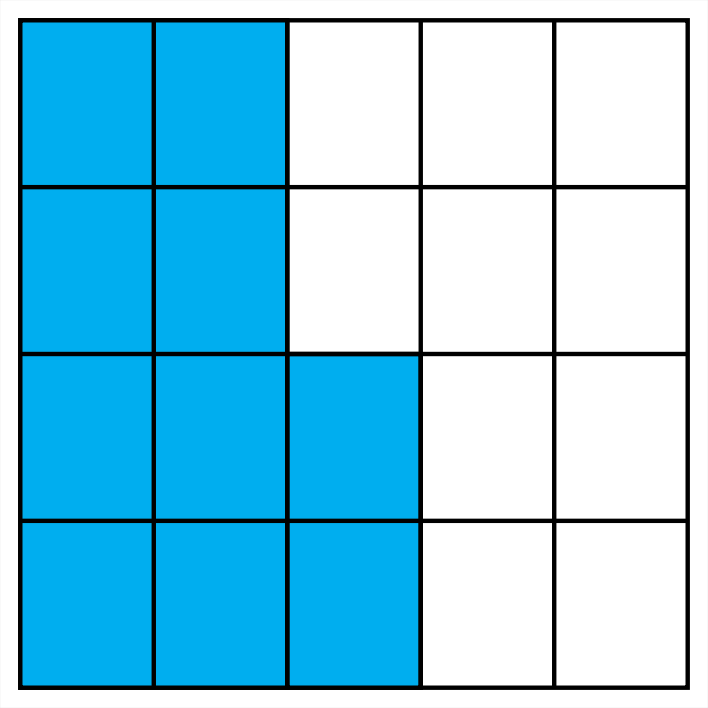
\includegraphics[width=45px]{../images/imagen_frac01.png} \fillin[\fbox{$\dfrac{10}{20}$}][0in] \\[1em]
				\part 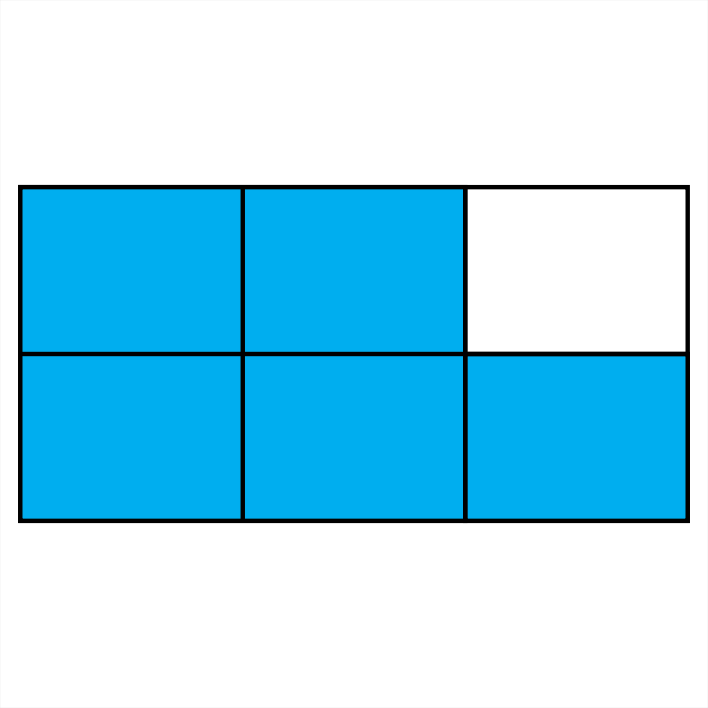
\includegraphics[width=45px]{../images/imagen_frac02.png} \fillin[\fbox{$\dfrac{5}{6}$}][0in] \\[1em]
				\part 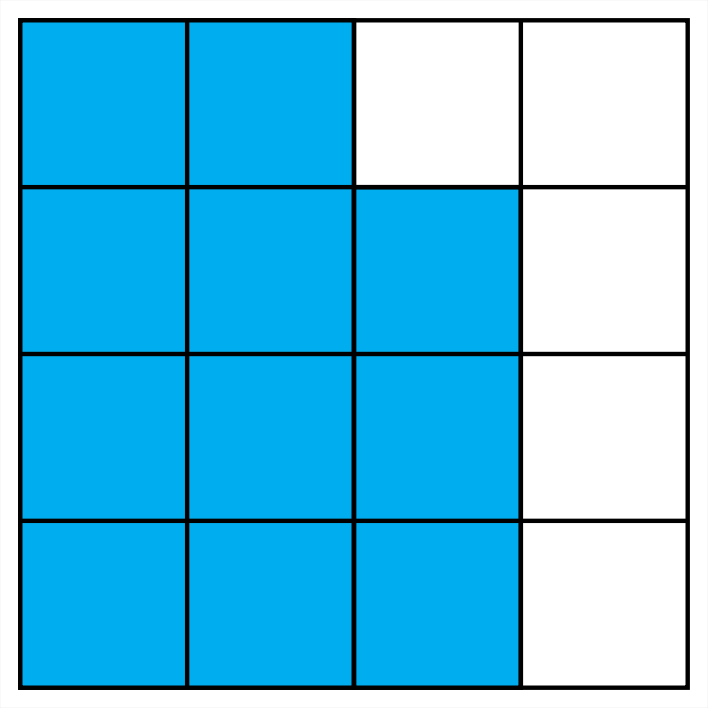
\includegraphics[width=45px]{../images/imagen_frac03.png} \fillin[\fbox{$\dfrac{11}{16}$}][0in] \\[1em]
				\part 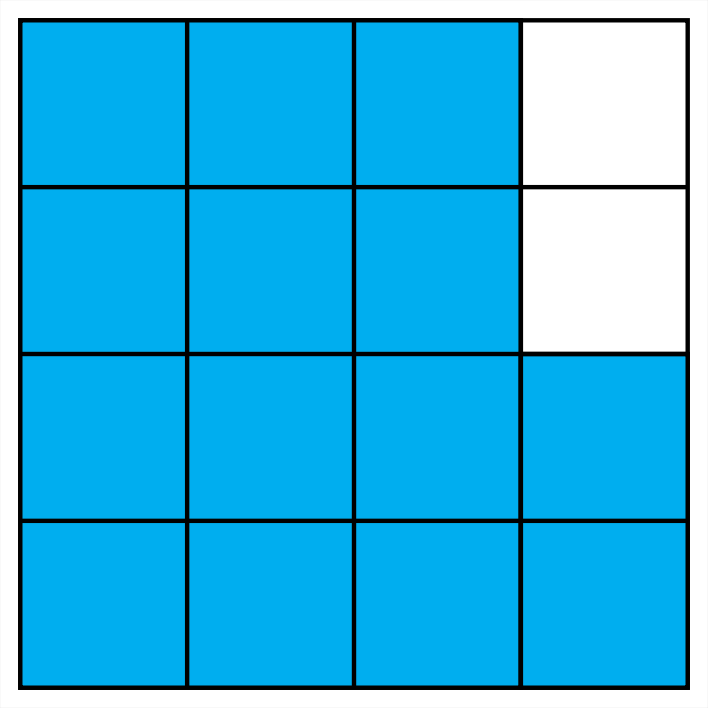
\includegraphics[width=45px]{../images/imagen_frac04.png} \fillin[\fbox{$\dfrac{14}{16}$}][0in] \\[1em]
				\part 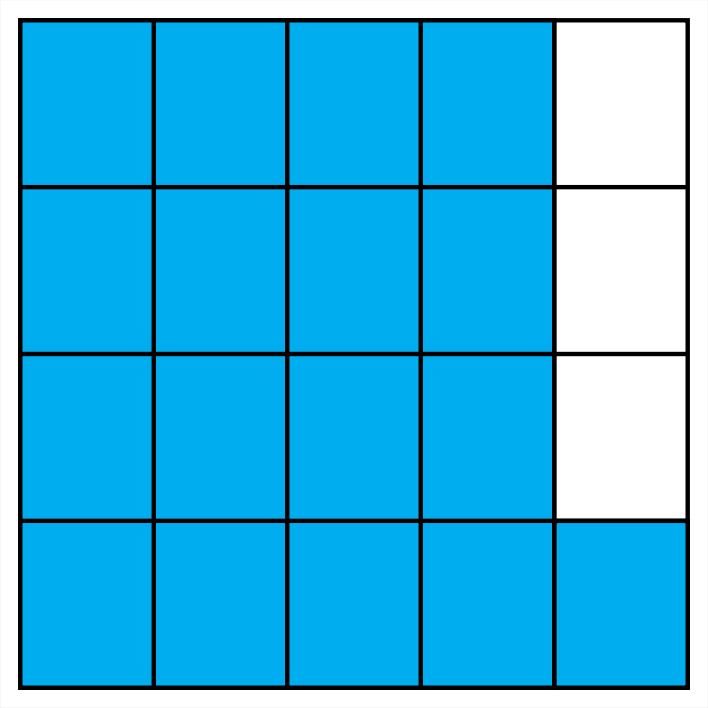
\includegraphics[width=45px]{../images/imagen_frac05.png} \fillin[\fbox{$\dfrac{17}{20}$}][0in] \\[1em]
				\part 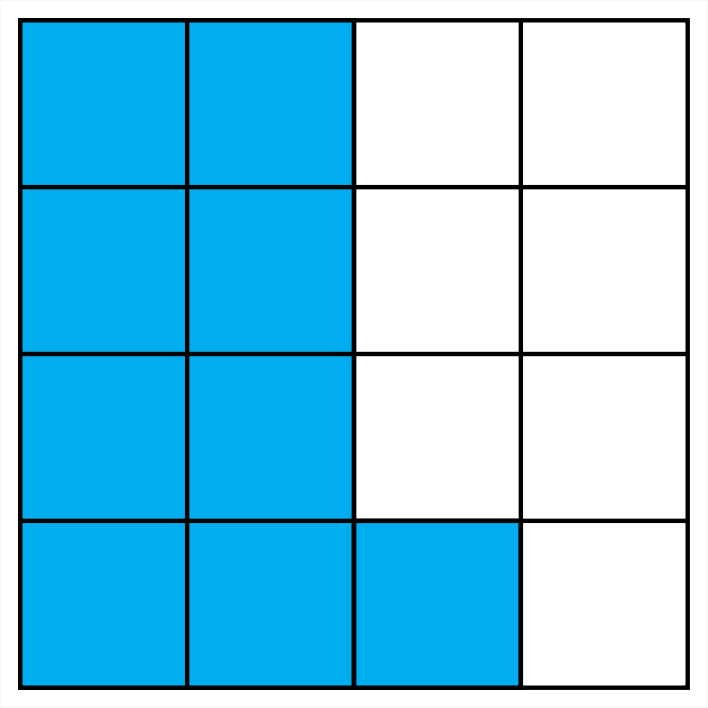
\includegraphics[width=45px]{../images/imagen_frac06.png} \fillin[\fbox{$\dfrac{9}{16}$}][0in] \\[1em]
				\part 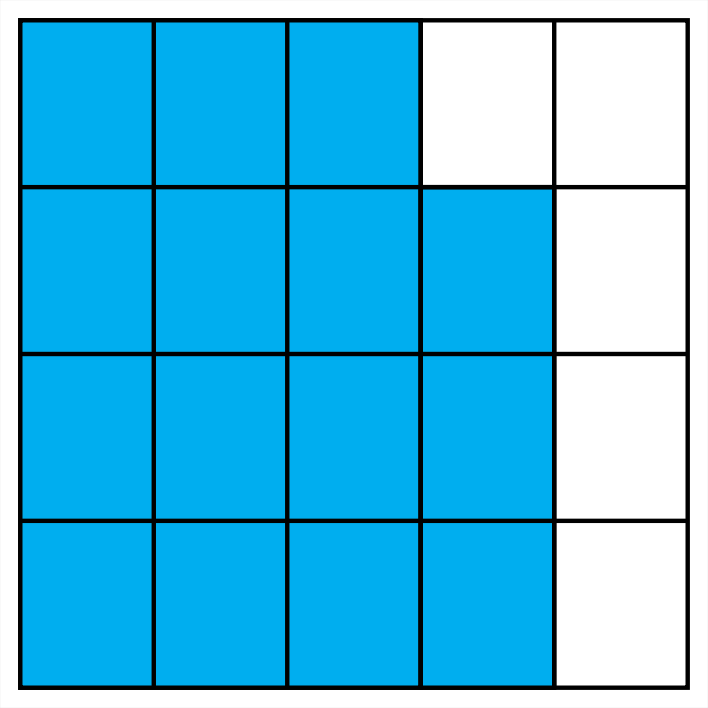
\includegraphics[width=45px]{../images/imagen_frac07.png} \fillin[\fbox{$\dfrac{15}{20}$}][0in] \\[1em]
				\part 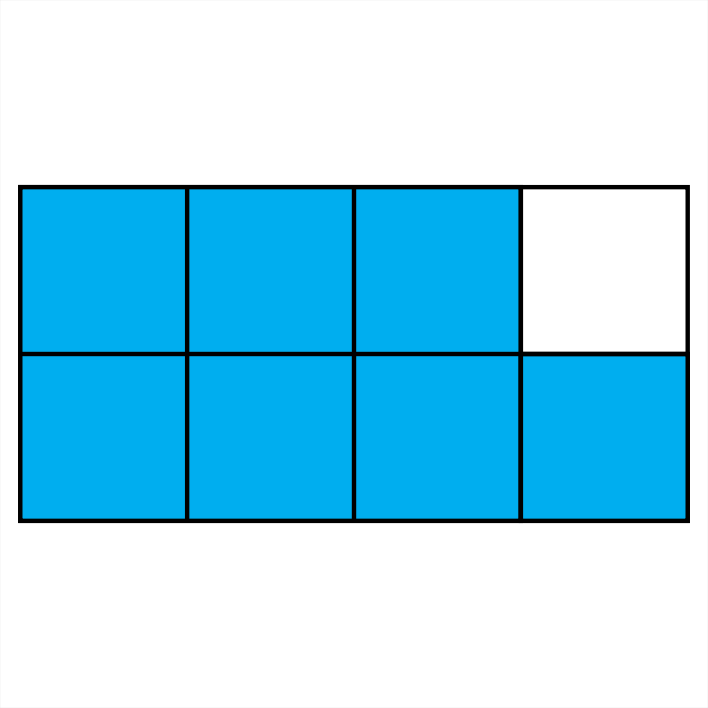
\includegraphics[width=45px]{../images/imagen_frac08.png} \fillin[\fbox{$\dfrac{7}{8}$}][0in] \\[1em]
				\part 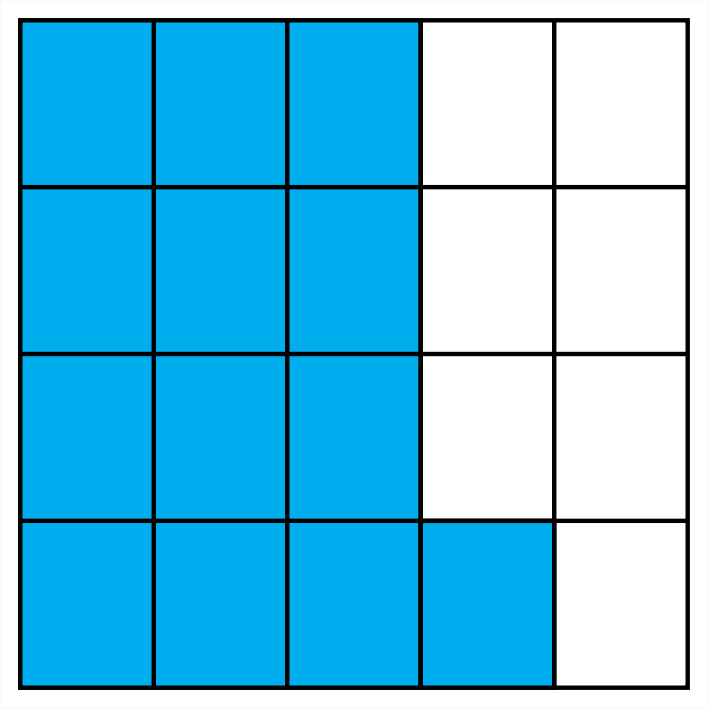
\includegraphics[width=45px]{../images/imagen_frac09.png} \fillin[\fbox{$\dfrac{13}{20}$}][0in] \\[1em]
				\part 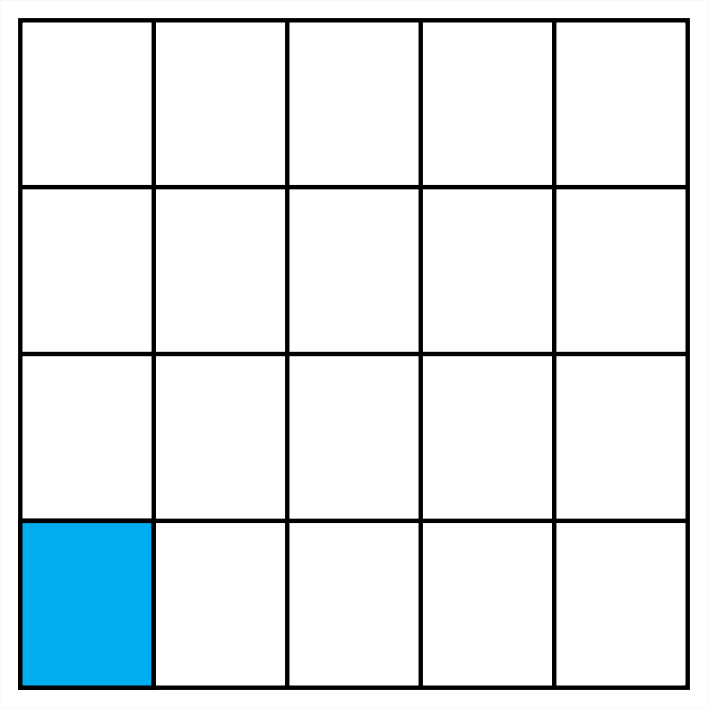
\includegraphics[width=45px]{../images/imagen_frac11.png} \fillin[\fbox{$\dfrac{1}{20}$}][0in] \\[1em]
			\end{parts}
		\end{multicols}
	}


	% \subsection*{\ifprintanswers{Nombre de fracciones                       }\else{}\fi}

	\questionboxed[5]{Escribe la fracción que corresponda en cada inciso:

		\begin{parts}
			\part ¿Cómo se escribe numéricamente la fracción \textbf{ocho quintos}?    \fillin[$\dfrac{8}{5}$][0in]  \\
			\part ¿Cómo se escribe numéricamente la fracción \textbf{seis onceavos}?   \fillin[$\dfrac{6}{11}$][0in] \\
			\part ¿Cómo se escribe numéricamente la fracción \textbf{dos séptimos}?    \fillin[$\dfrac{2}{7}$][0in]  \\
			\part ¿Cómo se escribe numéricamente la fracción \textbf{once medios}?     \fillin[$\dfrac{11}{2}$][0in] \\
			\part ¿Cómo se escribe numéricamente la fracción \textbf{diez décimos}?    \fillin[$\dfrac{10}{10}$][0in]\\
		\end{parts}
	}

	% \subsection*{\ifprintanswers{Conversión de fracciones mixtas a impropias}\else{}\fi}

	\questionboxed[3]{Convierte la siguientes fracciones mixtas a impropias:

		\begin{multicols}{3}
			\begin{parts}\large
				\part $4\dfrac{2}{3}= $ \fillin[$\dfrac{14}{3}$][0in]
				\part $2\dfrac{3}{10}= $ \fillin[$\dfrac{23}{10}$][0in]
				\part $5\dfrac{1}{5}= $ \fillin[$\dfrac{26}{5}$][0in]
			\end{parts}
		\end{multicols}
	}

	% \subsection*{\ifprintanswers{Conversión de fracciones impropias a mixtas}\else{}\fi}

	\questionboxed[3]{Convierte la siguientes fracciones impropias a mixtas:

		\begin{multicols}{3}
			\begin{parts}\large
				\part $\dfrac{13}{3}= $ \fillin[$4\dfrac{1}{3}$][0in]
				\part $\dfrac{63}{10}= $ \fillin[$6\dfrac{3}{10}$][0in]
				\part $\dfrac{51}{5}= $ \fillin[$10\dfrac{1}{5}$][0in]
			\end{parts}
		\end{multicols}
	}

	% \section*{\ifprintanswers{Operaciones con fracciones                 }\else{}\fi}
	% \subsection*{\ifprintanswers{Suma de fracciones                         }\else{}\fi}
	% \subsection*{\ifprintanswers{Resta de fracciones                        }\else{}\fi}
	% \subsection*{\ifprintanswers{Multiplicación de fracciones               }\else{}\fi}
	% \subsection*{\ifprintanswers{División de fracciones                     }\else{}\fi}
	% \subsection*{\ifprintanswers{Operaciones de fracciones mixtas           }\else{}\fi}

	\questionboxed[8]{Realiza las siguientes operaciones.

		\begin{multicols}{2}
			\begin{parts}\large
				\part $\dfrac{3}{5}+\dfrac{4}{5}=$ \fillin[$\dfrac{7}{5} = 1\dfrac{2}{5}$][0in] \\[2em]
				\part $\dfrac{13}{6}-\dfrac{5}{6}=$ \fillin[$\dfrac{8}{6}=\dfrac{4}{3}$][0in] \\[2em]
				\part $\dfrac{12}{7}-\dfrac{5}{7}=$ \fillin[$\dfrac{7}{7}=1$][0in] \\[2em]
				\part $1\dfrac{1}{8}+1\dfrac{7}{8}=$ \fillin[$2\dfrac{8}{8} = 3$][0in] \\[2em]
				\part $\dfrac{3}{5}\times\dfrac{2}{3}=$ \fillin[$\dfrac{6}{15}$][0in]   \\[2em]
				\part $\dfrac{7}{8}\times\dfrac{3}{4}=$ \fillin[$\dfrac{21}{32}$][0in] \\[2em]
				\part $\dfrac{3}{5} \divisionsymbol\dfrac{2}{3}=$ \fillin[$\dfrac{9}{10}$][0in] \\[2em]
				\part $\dfrac{7}{8} \divisionsymbol\dfrac{3}{4}=$ \fillin[$\dfrac{28}{24}$][0in]	\\[2em]
			\end{parts}
		\end{multicols}
	}
\end{questions}
\end{document}